\documentclass[12pt,a4paper,twoside,times,sky,standard]{csiroreport2017}

\usepackage[utf8]{inputenc}
\usepackage{amsmath}
\usepackage{amssymb}
\usepackage{hyperref}
\usepackage{dirtytalk}
\newcommand{\wh}{\widehat}
\newcommand{\ds}{\displaystyle}
\newcommand{\alp}{\alpha}
\newcommand{\bet}{\beta}
\newcommand{\gam}{\gamma}
\newcommand{\eps}{\epsilon}
\newcommand{\veps}{\varepsilon}
\newcommand{\etal}{\textit{et al.}}
\newcommand{\xmu}{\mbox{\boldmath$\mu$}}
\newcommand{\xtheta}{\mbox{\boldmath$\theta$}}
\newcommand{\xxi}{\mbox{\boldmath$\xi$}}
\newcommand{\xSigma}{\mbox{\boldmath$\Sigma$}}
\newcommand{\sigr}{\sigma^2_r}
\newcommand{\bmsy}{B_{\rm msy}}
\newcommand{\cmsy}{C_{\rm msy}}
\newcommand{\hmsy}{H_{\rm msy}}

\docdivision[Environment]


\docbusinessunit[
    CSIRO Environment\\
    Battery Point, Hobart 7000, Tasmania, Australia.\\
]


% The title of the document. Try to keep it to 3 lines or less.

\doctitle[\vspace{0mm}\huge Conditioning IOTC Albacore OMs using the ABC approach]

\docfootertitle[IOTC Albacore OMs]

\docauthors[\vspace{4mm}\large Rich Hillary\\ CSIRO Environment\\and\\ Iago Mosqueira \\Wageningen Marine Research, The Netherlands]

\docfurtherinfoA[CSIRO Environment]{Rich Hillary}{+61 3 6232 5452}%
{Rich.Hillary@csiro.au}{https://www.csiro.au/en/Research/Environment}{CSIRO Environment website}

\docfurtherinfoB[Wageningen Marine Research]{Iago Mosqueira}{+31 317 480 900}%
{iago.mosqueira@wur.nl}{https://www.wur.nl/en/research-results/research-institutes/marine-research.htm}{Wageningen Marine Research website}

%\docreportnum[Report Number: CMIS 2009/00]

%\docreportdate[18th June 2019]

\doccopyrightyear[2023] % For the Copyright and Disclaimer notice

\begin{document}
%=================================================

\section{Background}

For the current suite of IOTC MSE work, the general approach to conditioning the required set of Operating Models (OMs) has been to use the species-specific stock assessment model structure as the basis for the OMs. A grid of model runs, formulated using a set of alternative assumptions and inputs, is constructed based on the base case assessment model. In \cite{om21} an alternate, complementary approach was outlined where, instead of the assessment being the basis for conditioning, a suite of possible prior states of historical dynamics and current status are defined. The available, but mostly the more contemporary, data are included within an estimation scheme built on emerging Approximate Bayesian Computation (ABC) and Synthetic Likelihood (SL) concepts \cite{abc,synlkhd}. The aim is to generate a distribution of current abundance, mortality and status that is consistent with both the available data and the suite of possible prior states of nature defined beforehand. This can then be used to initialise the OMs used to project the stock into the future and test the candidate MPs.

A stock assessment, in this context, can be viewed as our attempt to do both of these things at once. Ideally, this is arguably a sensible option; however, it is not always successful. The ongoing struggles with the Yellowfin tuna stock assessment, and the conditioning of OMs based upon it, outline this problem: what if you cannot adequately reconcile the data, assessment model structures, and the resultant estimates of current status and future projected dynamics? In \cite{om21} we proposed an alternate approach arguing that using a stable, agreed and robust stock assessment was a natural first option, but that the ABC approach was a potentially viable - and scientifically pragmatic - alternative approach if the assessment route was unsuccessful.

In this paper we condition the Indian Ocean Albacore tuna OM that mirrors (biologically and structurally) the most recent stock assessment, utilises length composition and longline CPUE data, and is able to explore a wide range of stock status prior hypotheses, many of them built on information from the results of the stock assessment. The aim of this work was to cover the
same range of factors/hypotheses covered in the previous suite of OMs (REFS):

\begin{enumerate}
    \item Use of - and generation of data from - alternative CPUE series
    \item Influence of size data
    \item Impact of assumed catchability increases in LL fleets
    \item Uncertainty in steepness and natural mortality
    \item Uncertainty in recruitment variability
\end{enumerate}

\section{Methods}

ABC \cite{abc} and SL \cite{synlkhd} methods can be used to define an \emph{approximate} distribution for the parameters $\xtheta$ we are interested in; subsequently, we obtain an approximate distribution for all the variables that depend on those parameters. Where they differ from more classical frequentist or Bayesian methods is how the data, $D$, are included. Classical methods posit a likelihood for the data, given the parameters: $\ell\left(D\,|\,\xtheta\right)$; for a Bayesian analysis we then define a prior distribution, $\pi(\xtheta)$ to then obtain the posterior distribution of the parameters given the data:

\begin{equation*}
  \pi\left(\xtheta\,|\,D\right) = \frac{\ell\left(D\,|\,\xtheta\right)\pi(\xtheta)}{\pi(D)}
\end{equation*}

The ABC approach relaxes the requirement for a specific likelihood (i.e. data generating probability model) to the idea of a \emph{discrepancy} statistic that measures the difference between the observed data, and the model-derived process variables, $X$, that relate to it. The simplest example would be some distance metric $\rho(D,X)$ whereby we require that this distance between the observed data and our prediction is less than some value $\delta>0$ (i.e. assumes uniform error on a radius $\delta$). Values whereby $\rho(D,X)\geq\delta$ receive zero probability mass and, in a sampling scheme, would never be accepted. This simple approach will not necessarily work for certain types of data, especially the types we often have in fisheries contexts, but there are natural generalisations of this simple discrepancy idea.

The other very useful thing we can easily embed within a sampling scheme is informative priors on various elements of the process variables, $X$, which effectively imply a prior on the key parameters, $\pi(\xtheta)$. This means we can also define informative priors for the various stock status variables (MSY ratios, SSB depletion \textit{etc}.) and include the most relevant recent data, without having to fully model the historical dynamics and data and define appropriate likelihoods for these data. If we are departing from the stock assessment approach, this implies that we have not really succeeded in being able to robustly estimate the distribution of these key status variables. This approach takes a step back and instead tries to define scenarios (specifically distributional scenarios) for these variables at particular periods in time that are consistent with previous assessment experiences and the data. In terms of likely data sources, the two most obvious examples in tuna models are the CPUE indices of abundance, and the catch at length composition. For some examples we may also have mark-recapture data (e.g. tropical tuna) or other data sources. These can be naturally added to the algorithm, as long as the population and fishery model can generate observations for them and a distance metric can be computed.

The population models and associated biological relationships will be very similar to the stock assessment, given they need to have the same structure as the existing OMs (which we do not propose need changing at this stage). The main technical challenge is constructing the discrepancy statistics for the data, and the sampling scheme to generate samples from our approximate distribution of the parameter and population dynamic variables. We have moved the technical details of how these are done to Appendix A to avoid an unnecessary amount of technical exposition in the main body of the paper: what we are trying to demonstrate is that we can get the variables we need for OM conditioning, using plausible status scenarios, key data sets and emerging powerful statistical sampling techniques.

\section{Albacore case study}

The basis for the models and data explored in the Albacore example is contained in the most recent stock assessment \cite{albsa}. In terms of model structure, the model is setup as follows:

\begin{itemize}
    \item Annually structured but with four annual seasons and recruitment in a single pre-specified season.
    \item No explicit spatial structure but with the same areas-as-fleets approach as the stock assessment.
    \item Sexually-structured population dynamics driven by growth and selectivity-at-age (selectivity-at-length is not sexually structured by fishery).
    \item Time-frame for conditioning is 2000 -- 2020, so as to model all surviving cohorts.
    \item Model considers 4 long-line fleets, 1 \emph{other} fleet and 1 purse seine fleet. The 16 seasonal long-line fleets are condensed into 4 fleets, each with 4 seasons of catch, effort and size data (e.g. LL1 is fisheries 1-4 in the assessment).
    \item A Beverton \& Holt steepness-unfished recruitment stock-recruit relationship is used with lognormally distributed deviations constrained by a pre-specified $\sigma_r=0.3$, as per the assessment \cite{albsa}.
\end{itemize}

The stock assessment model fits to the disaggregated length-frequency data and the seasonal CPUE data from the longline fleets. The initial approach taken in the ABC albacore modelling was not to fit to disaggregated length frequency data, which is very variable and noisy from season to season and year to year. Instead, we aggregate the size data across years and seasons and fit to a mean size frequency data set per fishery. The reason behind this choice is to obtain a representative selectivity relationship for each fishery, and give a clear indication of the average size structure in the fisheries over the time period. Additionally, it purposefully reduces the influence of the size data on the overall population abundance scale, which is a known issue already considered in the previous OM grid.

\subsection{Stock status priors}

These status priors are a key feature of the OM conditioning methodology we propose. To constrain both absolute and relative abundance, as well as fishing pressure we explore a range of possible types (and parameterisations) of status prior. The following four general types are explored (in different forms):

\begin{enumerate}
    \item Relative SSB: the most general status variable ($SSB_y/SSB_0$) - for any range of years we allow a prior mean and SD
    \item SSB MSY ratio: the ratio of SSB to that at MSY ($SSB_y/SSB_{\rm msy}$) - for any range of years we allow a prior mean and SD
    \item Harvest rate MSY ratio: the ratio of fleet-averaged harvest rates to MSY levels - for any range of years we allow a prior mean and SD
    \item Overfishing probability: if the harvest rate exceeds the level at MSY a half-normal penalty can be applied to penalise against trajectories with very high harvest rates (and likely will crash early in the projections)
\end{enumerate}

The status priors are based on information reported in the most recent stock assessment \cite{albsa}. Different combinations of status priors are employed for different OM conditionings to explore a balance between letting the data inform the model (w.r.t. abundance indices), and forcing the OMs to adhere closer to the assessment outcomes. For relative SSB we define a prior for the first year (2000) centered on 0.5 with a 95\% prior CI of 0.3--0.7. For the relative SSB MSY ratios we define a prior for the last two years (2019 and 2020) centered on 2.25 and 2 with an SD of 0.35 for both. For the scenarios where we apply a prior on the harvest rate MSY ratios for the first and last years (2000 and 2020) we assign a prior mean of 0.6 with an SD of 0.2 (so a prior range of around 0.2--1). These are used for scenarios where it is clear there is no information in the abundance indices in relation to population scale. Applying these vaguely informative priors penalises against scenarios where there is effectively no effect of fishing on abundance, the population is very very large and the abundance trends are recruitment driven. When the overfishing probability penalty is applied - to avoid overly pessimistic individual runs - it is applied for all years and where the probability of the overfishing ratio exceeding 2 is less than or equal to 0.05.

\subsection{Covariant prior for steepness and natural mortality}

A common, and fair, criticism of many stock assessments is that they often have fixed values of both steepness and natural mortality. One of the main outcomes of this is that we effectively fix the MSY variables - especially the stock status ratios for both SSB and fishing mortality \cite{steepm}. The factorial grid approach tries to address this issue by exploring a combination of discrete values for both parameters. A major drawback of this approach is that it is not \textit{a priori} able to avoid combinations of these two parameters that result in pathologically over/under resilient stock-recruit relationship dynamics. More specifically, for the IOTC a common issue seems to be combinations that are overly pessimistic, resulting in population trajectories that very quickly end up crashing (ALB MSE refs).

Generally speaking, higher/lower values of steepness/natural mortality will tend to result in similar MSY ratios; high/low values of both are often overly optimistic/pessimistic. We attempt to utilise this inter-relationship to construct a covariant joint prior for these two parameters from which we will sample in the ABC-MCMC algorithm outlined later on. The algorithm proceeds as follows:

\begin{enumerate}
    \item Define marginal distributions for both $h$ and $M$
    \item Calculate SSB depletion, $\tilde{\Delta}$, at MSY for expected values of $h$ and $M$
    \item Simulate $h$ and $M$ from their marginal distributions
    \item Define a tolerance interval $\veps$
    \item Only accept combinations of $h$ and $M$ within $\veps$ of $\tilde{\Delta}$
    \item Calculate correlation coefficient in retained bivariate samples
\end{enumerate}

This makes it possible to then define a bivariate normal distribution for h and M using the marginal variances and the estimated correlation coefficient from the algorithm described above. This then gives us a distribution of values from both h and M with the required marginal variances and a covariant structure that ensures we obtain internally consistent (with respect to MSY ratios) samples that are neither too optimistic or pessimistic relative to the expected MSY ratios.

For this example we take mean values of $h = 0.8$ for steepness and annual $M = 0.3$ as per the most recent stock assessment \cite{albsa}. We calculate an SD for steepness that results in a prior 95\% CI of 0.7--0.9; for $M$ we define a 5\% CV so that the prior 95\% CI is 0.27--0.33. Using the correlation estimation algorithm described above with a tolerance of $\veps = 5\%$ we obtained a correlation coefficient of -0.58.

\subsection{OM scenarios}

As stated previously, one of the main intentions of this work is to at least be able to cover all the main axes of uncertainty covered in previous Indian Ocean Albacore OM conditioning:

\begin{enumerate}
    \item Steepness and natural mortality: covariant joint prior now integrated into the ABC-MCMC algorithm
    \item Recruitment variance: alternative OM conditioning that now actively estimates the recruitment variance, $\sigr$ , with an informative prior with mean 0.3 and prior 95\% CI of 0.2--0.5
    \item Weighting of size data: the issue was their influence on the estimates of population scale. By aggregating the size data across years and seasons, and establishing a conservative weighting strategy in the ABC discrepancy function, we have effectively removed this as an issue
    \item Longline catchability trends: we explore a 1\% \textit{per annum} increasing trend in the longline CPUE series in alternative OM conditioning runs
    \item CPUE series: we explore using the seasonal CPUE indices from longline fleets 1 and 3 - not jointly but separately to avoid data conflicts that will not be resolved without more complex spatially structured models
\end{enumerate}

\section{Results}

The key OM stock status variables we summarise are relative SSB, $\Delta_y=SSB_y/SSB_0$, SSB relative to MSY, $\tilde{\Delta}_y=SSB_y=SSB_y/SSB_{\rm msy}$, and harvest rate relative to MSY, $\mathcal{H}_y=H_y/H_{\rm msy}$. The seven different OM conditioning scenarios are:

\begin{itemize}
    \item \textbf{R1}: Uses CPUE from LL fleet 1 with SSB priors but no harvest rate priors
    \item \textbf{R1a}: Uses CPUE from LL fleet 3 with SSB and harvest rate MSY priors
    \item \textbf{R1b}: Uses CPUE from LL fleet 1 with SSB and overfishing probability priors
    \item \textbf{R2}: Same as R1 but $\sigr$ is estimated 
    \item \textbf{R2a}: Same as R1a but $\sigr$ is estimated
    \item \textbf{R3}: Same as R1 but assumes 1\% increasing catchability trend
    \item \textbf{R3a}: Same as R1a but assumes 1\% increasing catchability trend
\end{itemize}

Before outlining the results it will be helpful to focus on the important qualitative differences between the OM scenarios. Table 4.1 summarises the status of each of the seven OM conditioning scenarios described above. Scenario R1 is arguably where the data - specifically the CPUE abundance indices - have the most influence of both population scale and abundance, biomass and mortality trends. Scenarios R1a, R2a, and R3a are all penalised to be close to the high-level stock status summaries coming from the stock assessment \cite{albsa} - in particular the harvest rate MSY ratio priors in the first and final years are applied in these cases. The reason for this is because of the lack of information in the CPUE from fleet 3 in relation to population scale and an apparent production function emerging from the models. For these runs we saw intermittent very high abundance samples (i.e. a very skewed right-hand tail in the $R_0$ posterior distribution) where the trends in abundance were just as easily explained by recruitment variability versus fishing pressure. As a result, the relative SSB estimates are still concordant with the status priors but fishing mortality is effectively zero for these samples. By applying not just the biomass-based status priors but additionally the harvest rate MSY ratio priors (scenarios Rxa) we avoided these pathological very high abundance runs because the harvest rates could not reduce to such low levels a priori. This is not, perhaps, surprising given the apparent lack of correlation between abundance trends and overall catch biomass - this is quite different for the fleet 1 CPUE and the results attest to this fundamental difference between the two fleet CPUE indices. For the R1b run the overfishing probability penalty was applied due to the appearance of high levels of overfishing in certain runs in the last 5 years of the model time-frame. As already
stated, if we do not penalise against these runs they are likely to result in rapid declines in abundance in the first years of the projections at current catch levels. As can clearly be seen from Table 4.1 applying this prior does not really change the biomass status results, but it does avoid the high levels of overfishing in the final conditioning years. What this overfishing penalty does is to increase the correlation between the various parameters and avoid those combinations that result in very high overfishing rates. The 1\% p.a. increasing trend in catchability scenarios (R3 \& R3a) results in slightly lower median biomass ratios by the end of the modelling time-frame, stronger overall declines in abundance over the time-frame, and most clearly the lowest/highest quantiles of the status ratios - depending on the ratio and what quantile is pessimistic relative to the median - are lower/higher for these scenarios.

\begin{table}[hb]
    \begin{center}
        \begin{tabular}{|ccccc|}
            \hline
            OM scenario & $\Delta_{2000}$ & $\Delta_{2020}$ & $\tilde{\Delta}_{2020}$ & $\mathcal{H}_{2020}$\\
            & & & & \\
Prior & 0.5 (0.3-0.7)    & n/a              & 2 (1.3-2.7)      & 0.6 (0.2-1) \\
R1    & 0.76 (0.61-0.97) & 0.41 (0.22-0.56) & 1.9 (1.02-2.58)  & 1.13 (0.5-3.78) \\
R1a   & 0.56 (0.4-0.72)  & 0.48 (0.3-0.69)  & 2.01 (1.42-2.61) & 0.68 (0.33-1.38) \\
R1b   & 0.74 (0.61-0.9)  & 0.42 (0.24-0.54) & 1.98 (1.16-2.49) & 0.98 (0.46-2.4) \\
R2    & 0.71 (0.57-0.84) & 0.41 (0.21-0.55) & 1.91 (0.99-2.53) & 1.22 (0.45-3.57) \\
R2a   & 0.56 (0.41-0.72) & 0.47 (0.28-0.71) & 2.03 (1.3-2.54)  & 0.65 (0.34-1.4) \\
R3    & 0.78 (0.6-0.91)  & 0.38 (0.15-0.52) & 1.77 (0.7-2.44)  & 1.4 (0.58-5.06) \\
R3a   & 0.63 (0.48-0.77) & 0.42 (0.25-0.59) & 1.94 (1.23-2.5)  & 0.71 (0.35-1.45) \\
            & & & & \\
            \hline
        \end{tabular}
    \end{center}
    \caption{\textit{Overall OM conditioning status summary in terms of the approximate posterior median and 95\% credible interval in brackets. Note the harvest rate MSY ratio is only applied in the Rxa scenarios; the overfishing probability is only applied for the Rxb scenarios.}}
\end{table}

\subsection{Fits to the data inputs}

The main difference in the scenarios with respect to which CPUE data that is used: quarterly
abundance indices from fleet 1 or fleet 3. In both cases we assume a seasonal structure to the
catchability parameters - this results in clear improvements in the fits to the data in both cases
but especially for the fleet 3 scenario. Clearly from Table 4.1, the choice of CPUE series has a
clear effect on all the status levels and trends. However, the fits to the data are not meaningfully
affected by either estimating $\sigr$ or the assumption of a 1\% annual increasing catchability trend,
so we only graphically display the fits to the CPUE data for scenarios R1 and R1a in Figure 4.1.
For fleet 1 the abundance trends are arguably best captured in seasons 1 and 4 with very few
observations outside the 95\% predictive intervals. For fleet 2 seasons 1, 3 and 4 seem to be the
best explained with the model struggling to fully capture the up and down trend in season 2. The
difference is not great, but in general the OMs seem to fit better to CPUE from fleet 1 versus that
from fleet 3.

\begin{figure}[hb]
    \begin{center}
        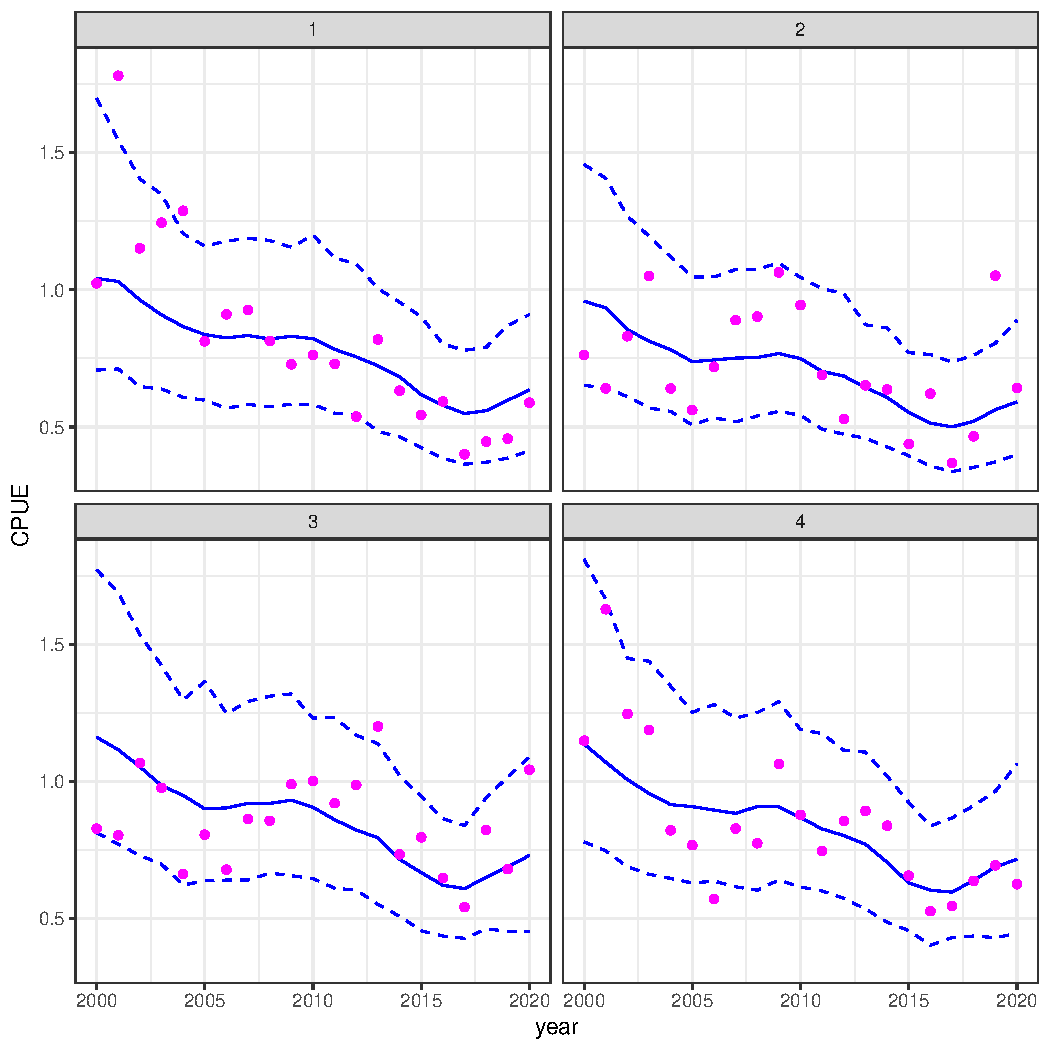
\includegraphics[width=7cm,height=7cm]{figs/case4_cpuefits.pdf}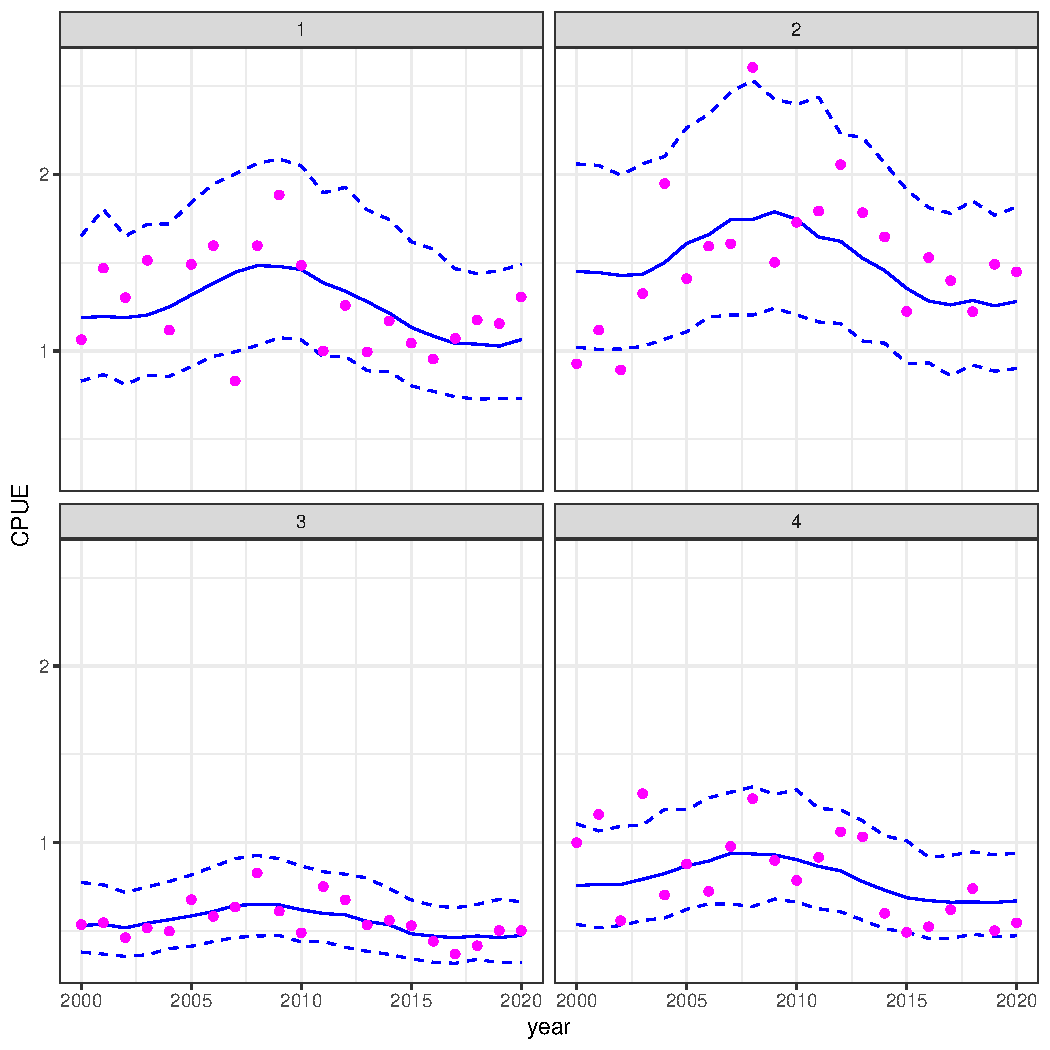
\includegraphics[width=7cm,height=7cm]{figs/case4a_cpuefits.pdf}
    \end{center}
    \caption{\textit{Fits to quarterly CPUE data (magenta circles) in terms of approximate posterior
median and 95\% credible interval (blue full and dotted lines) for fleet 1 (left) and 3 (right). In both
cases seasonal catchability parameters are estimated.}}
\end{figure}

As with the CPUE series scenarios, the fits to the size data are not obviously different when
estimating $\sigr$ or including catchability trends, so in Figure 4.2 we compare the fits to the size
data for scenarios R1 and R1a only. For all the five fisheries with size data (aggregated across
seasons and years) we see an acceptable fit to the length observations. Generally speaking, the
fits in scenario R1 (fleet 1 CPUE) are moderately better than those for R1a (fleet 3 CPUE). In
both scenarios the length data are the same, but Figure 4.3 shows the comparative selectivity-
at-length relationships for both scenarios. There are some subtle differences for 2, 3 and 4 but
no major ones - this suggests that the differences in the fit to the length data is attributable at
some level to the other key population dynamic and fishery variables in the model.

\begin{figure}[hb]
    \begin{center}
       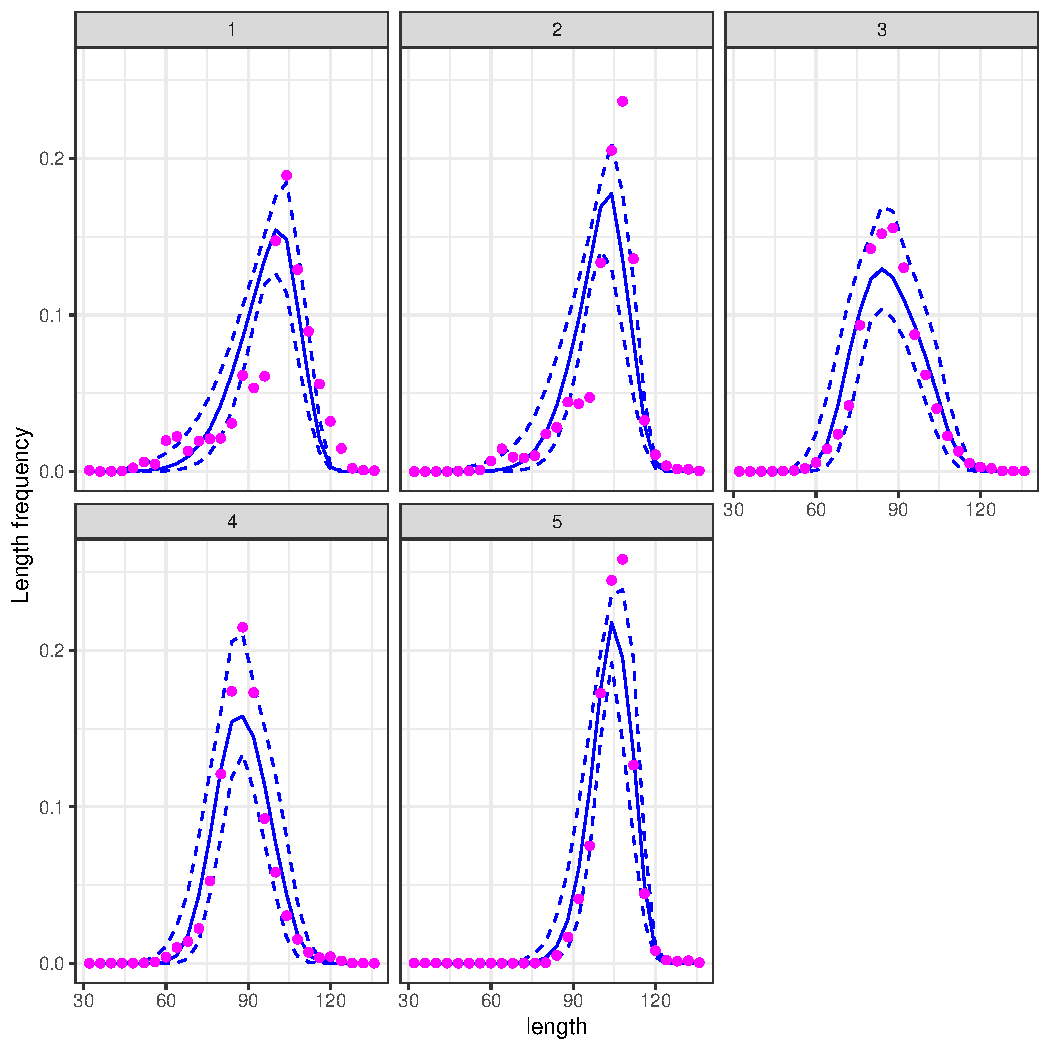
\includegraphics[width=7cm,height=7cm]{figs/case4_lffits.pdf}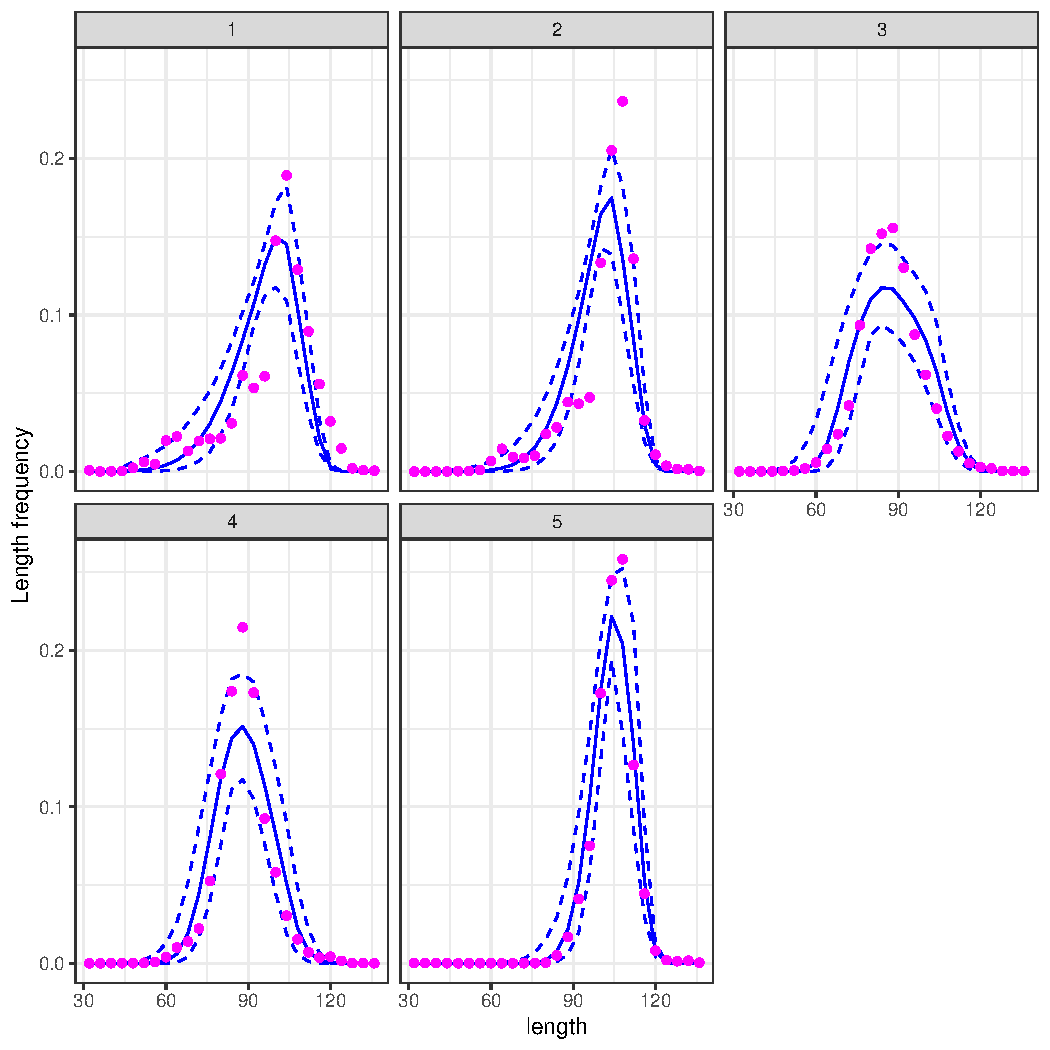
\includegraphics[width=7cm,height=7cm]{figs/case4a_lffits.pdf} 
    \end{center}
    \caption{\textit{Fits to aggregated length data (magenta circles) in terms of approximate posterior
median and 95\% credible interval (blue full and dotted lines) for fleet 1 (left) and 3 (right).}}
\end{figure}

\begin{figure}[hb]
    \begin{center}
       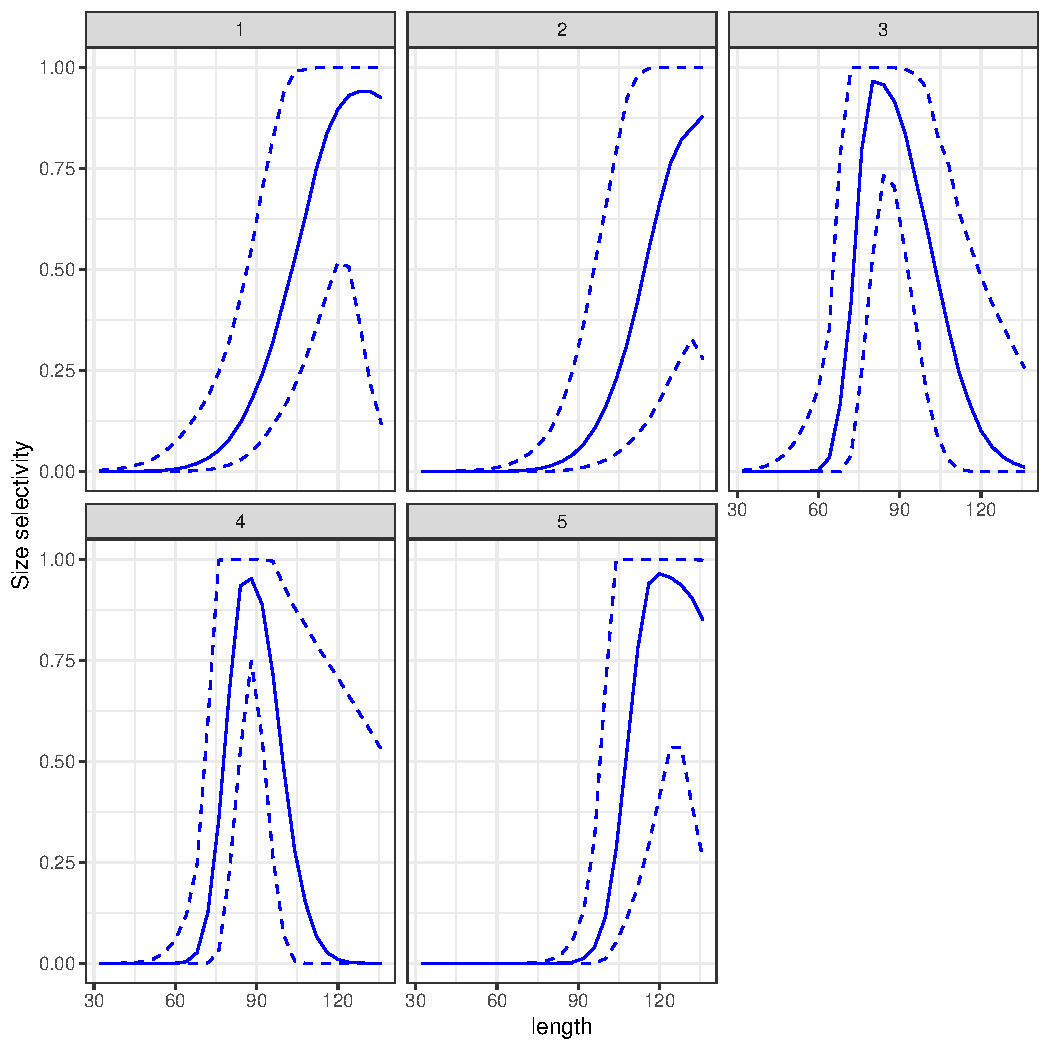
\includegraphics[width=7cm,height=7cm]{figs/case4_lengthsel.pdf}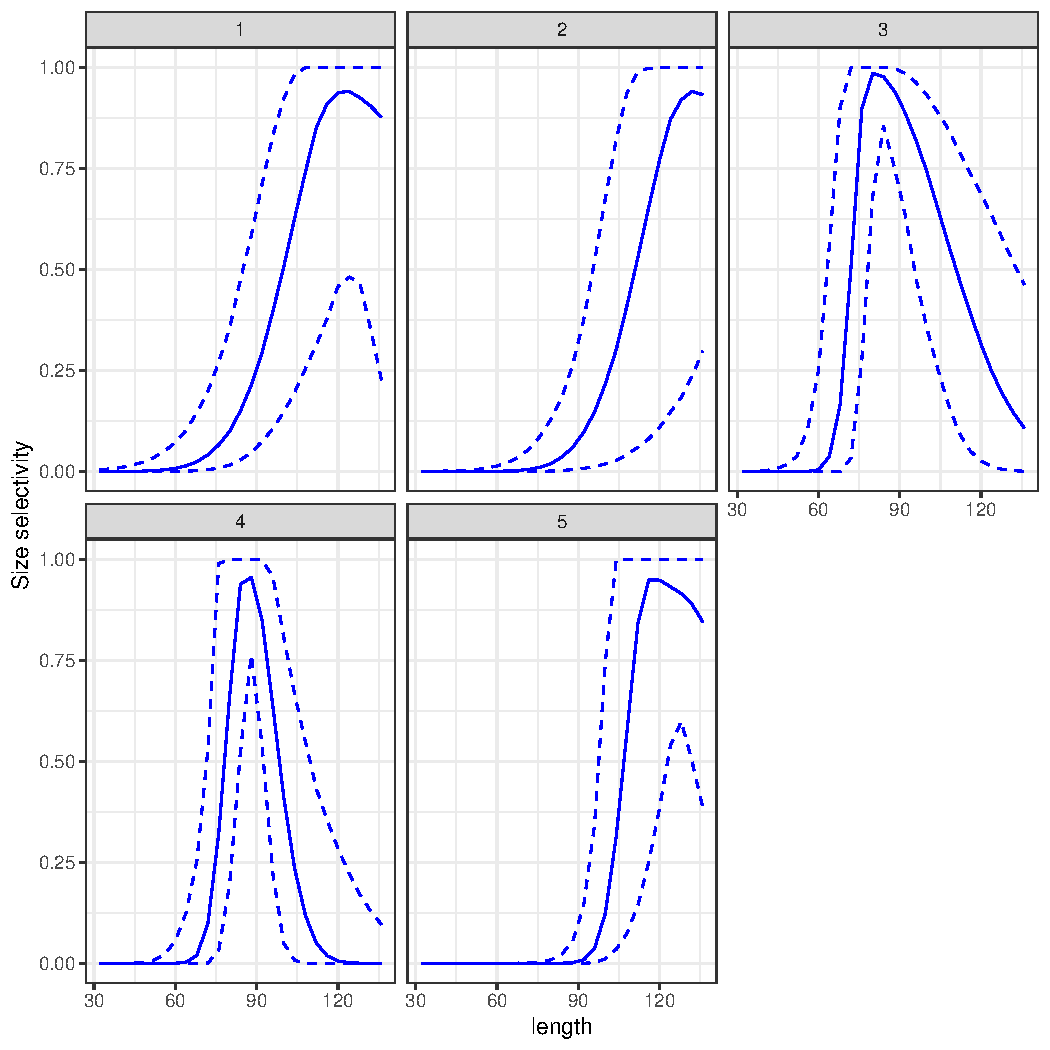
\includegraphics[width=7cm,height=7cm]{figs/case4a_lengthsel.pdf} 
    \end{center}
    \caption{\textit{Selectivity (assumed double normal) relationships-at-length for each fishery with
length data: blue line is the median and the dotted blue lines are the 95\% credible intervals.}}
\end{figure}

\subsection{Estimates of $\sigr$}

Runs R2 and R2a both explored the estimation of the recruitment variance parameter via the
conjugate prior approach outlined in the Appendix. The informative prior (assumed inverse-
Gamma) parameters where chosen to give a prior mean of 0.3 (value assumed in the assessment) and 95\% credible interval between 0.2 and 0.5. The aim was not to definitely estimate this parameter but to see, when given the freedom to deviate from the assumed value, was there strong information in the data. The prior and posterior distributions for $\sigr$ for both these OM scenarios can be seen in Figure 4.4. For the R2 scenario the posterior median (and 95\% credible interval) was 0.41 (0.26--0.63); for the R2a case it was 0.31 (0.23--0.47). For the R2 scenario the posterior estimates of $\sigr$ were higher than assumed in the assessment or the prior distribution employed herein. However, there is considerable overlap in the prior and posterior distributions and the impact on the key high-level status summaries of this increase in recruitment variability was minimal (see Table 4.1). For the R2a scenario there was little to no change in the overall posterior median relative to the prior - the only obvious change was an increase in the precision of $\sigr$ in the posterior. This is a clear signal that the data in this scenario are clearly very compatible with the underlying assumed value of 0.3 in the assessment.

\begin{figure}[hb]
    \begin{center}
       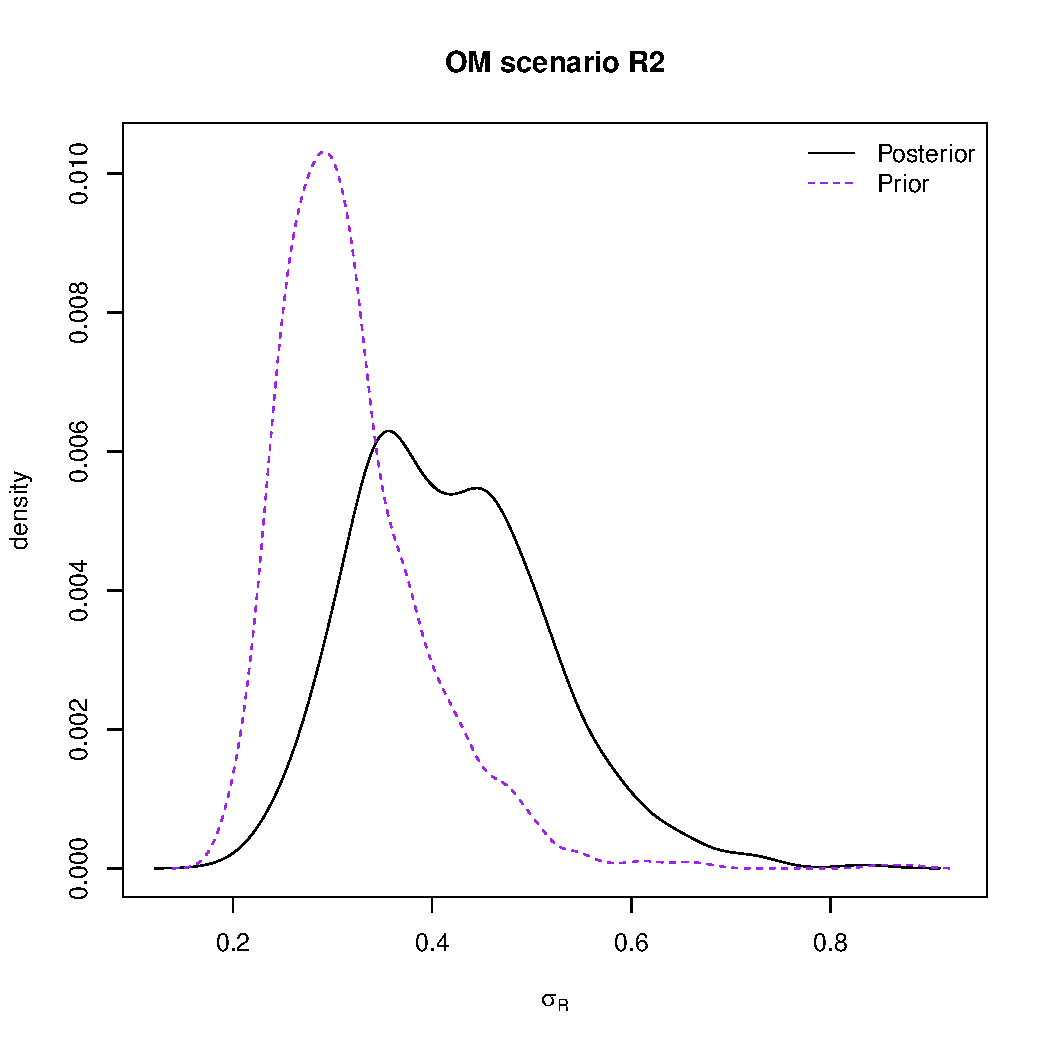
\includegraphics[width=7cm,height=7cm]{figs/pvsp_sigmar_R2.pdf}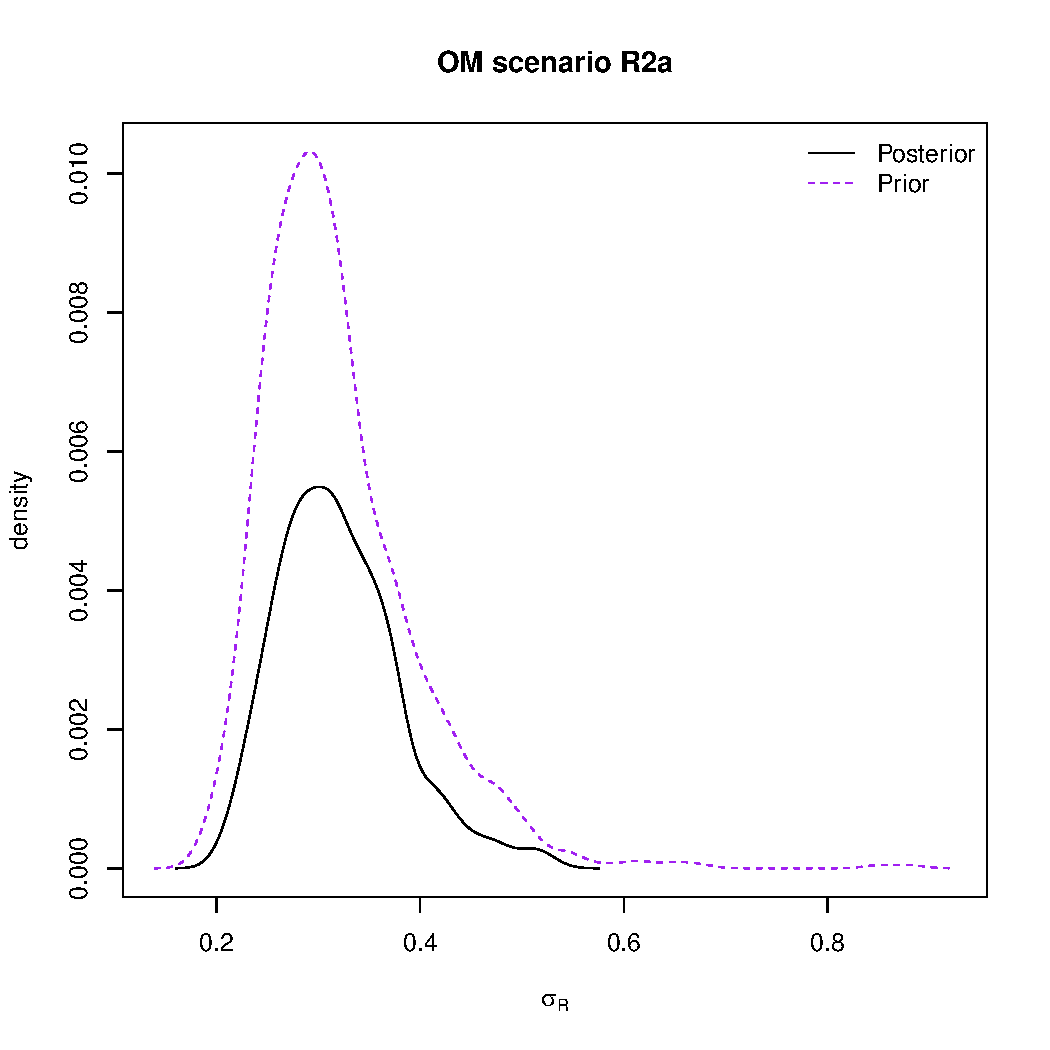
\includegraphics[width=7cm,height=7cm]{figs/pvsp_sigmar_R2a.pdf} 
    \end{center}
    \caption{\textit{Prior (dotted purple line) and posterior (full black line) for $\sigr$ for OM scenarios R2 (left) and R2a (right).}}
\end{figure}

\section{Discussion}

This paper outlines a full conditioning of a suite of OMs for Indian Ocean Albacore based on ideas originally raised in \cite{om21} and further explored in \cite{om23a}, with respect to methods for conditioning OMs that are not built upon the stock assessment model structures and output. The approach uses much, if not all, of the same demographic and life-history parameters the assessment does, and often key subsets of the same data if they are required to be simulated in the OMs. It also includes key prior information on current/recent/historical status variables (MSY ratios, depletion \textit{etc.}) to help estimate the main abundance, biomass and mortality variables required in the OMs. There is already an IOTC precedent for these type of approach - the original Skipjack tuna OM was conditioned in a similar fashion \cite{skj} using the methodology outlined in \cite{fst}.

THIS IS WHERE I GOT TO BEFORE PUSHING TO THE REPOS

\section{Acknowledgements}

Work by RH was funded by the Department of Foreign Affairs and Trade of the Government of Australia. Work by IM was funded by the Indian Ocean Tuna Commission (IOTC/FAO).

\clearpage
\begin{thebibliography}{99}
       
    \bibitem{om21} Hillary, R., Mosqueira, I., Preece, A., Rosa, D., Williams, A. and Edwards, C. (2021) Strategies for the conditioning of operating models for IOTC stocks, \textit{IOTC--2021--WPM12--16}
    
    \bibitem{abc} Sunnaker, M., Busetto, A., Numminen, E., Corander, J., Foll, M., \etal~(2013). Approximate Bayesian Computation. \textit{PLoS Comput. Biol.} {\bf 9}(1):e1002803. doi:10.1371/journal.pcbi.1002803.
         
    \bibitem{synlkhd} Wood, S. (2010) Statistical inference for noisy nonlinear ecological dynamic systems. \textit{Nature}. {\bf 466}: 1102--1107. doi: 10.1038/nature09319.

    \bibitem{albsa} Rice, J. (2022) Stock assessment of albacore tuna (\textit{Thunnus alalunga}) in the Indian Ocean using Stock Synthesis. \textit{IOTC--2022--WPTmT08--09}.

    \bibitem{steepm} Mangel, M. \etal~(2013) A perspective on steepness, reference points, and stock assessment. \textit{Can. J. Fish. Aquat. Sci.} {\bf 70}: 930--940.

    \bibitem{abcmcmc} Wilkinson, R. D. (2013) Approximate Bayesian Computation (ABC) gives exact results under the assumption of model error. \textit{Stat. Appl. Genet. Mol. Biol.} {\bf 12}(2): 129--141.
    
    \bibitem{mcmc} Brooks, S., Gelman, A., Jones, G., and Meng, X.-L. (1993) Handbook of Markov Chain Monte Carlo. \textit{Chapman \& Hall/CRC}.

    \bibitem{om23a} Hillary, R.M, and Mosqueira, I. (2023) Exploring the ABC approach for IOTC Albacore
        OM conditioning. \textit{IOTC--2023--MSETaskForce}
    
    \bibitem{skj} Bentley, N., and Adam. S. (2016) Management strategy evaluation for the Indian Ocean skipjack tuna fishery. Working paper IOTC-2016-WPM07-15 Rev1 presented to the 7 th IOTC Working Party on Methods, Mahe, Seychelles 11-13 November.
    
    \bibitem{fst} Bentley, N. and Langley, A. (2011). Feasible stock trajectories: a flexible and efficient sequential estimator for use in fisheries management procedures. \textit{CJFAS}. {\bf 69}(1): 161--177  

    \bibitem{kl} Kullback, S., and Leibler, R. A. (1951) On information and sufficiency. \textit{Annal. Math. Stats.} {\bf 22}: 79--96.

\end{thebibliography}

\clearpage
\section*{Appendix A}

\subsection*{Approximate McMC ABC algorithm}

There are a wide variety of possible algorithms that can be used to generate a sample from the approximate posterior distribution \cite{abc,synlkhd,abcmcmc}. Given the relative complexity of our likely suite of models, we consider that Algorithm D from \cite{abcmcmc} is the most applicable. It is basically an ABC-configured Metropolis-Hastings accept-reject algorithm as used in classic Bayesian McMC contexts. At time $t$, we have our joint parameter and process variable state $\Xi_t=\{\xtheta_t,X_t\}$. We generate a proposal for a new parameter vector $\xtheta^\prime$ (and $X^\prime=f(\xtheta^\prime)$) from the pre-specified transition kernel $q(\xtheta_t,\xtheta^\prime)$. We define the following acceptance probability for $\Xi^\prime=\{\xtheta^\prime,X^\prime\}$:

\begin{equation*}
    \ds \alpha(\Xi_t,\Xi^\prime)=\min\left(1,\frac{\pi(D,X^\prime)q(\xtheta^\prime,\xtheta_t)\pi(\xtheta^\prime)}{\pi(D,X_t)q(\xtheta_t,\xtheta^\prime)\pi(\xtheta_t)}\right)
\end{equation*}

and generate a random variable $u\sim U[0,1]$. If $\alpha(\Xi_t,\Xi^\prime)>u$ we accept the proposal and $\Xi_{t+1}=\Xi^\prime$; if $\alpha(\Xi_t,\Xi^\prime)\leq u$ we reject the proposal and set $\Xi_{t+1}=\Xi_t$. By choosing a symmetric normally distributed transition kernel $q(\xtheta_t,\xtheta^\prime)=q(\xtheta^\prime,\xtheta_t)$ this term disappears from the acceptance rate calculations. The prior distribution, $\pi(\xtheta)$, is for the estimated parameters. The $\pi(D,X^\prime)$ term is our likelihood analogue or discrepancy function - it includes both the observed data (catch length composition, abundance indices) and our additional information on the key status variables contained in the suite of process variables, $X$ (e.g. MSY and depletion ratios). The Markov chain transition kernels $q()$ are defined to use the random walk approach for sampling the posterior surface. To make the McMC algorithm more efficient we implement a Metropolis-within-Gibbs sampling approach \cite{mcmc}, where parameters are grouped together depending on expected correlation. Each block is updated using the Metropolis-Hastings algorithm, conditional on the parameters not included in that block being fixed at their most recent value. After doing this for each block of parameters (the Gibbs sampling part of the algorithm) we have fully updated all the parameters of the model and repeat the same process many times. Random walk variances are adjusted to achieve acceptance rates around 40\% - generally considered as optimally efficient \cite{mcmc}. A suitable burn in period is used to get the sampler moving on the surface before we decide to keep the samples, and these are then thinned to remove autocorrelation in the Markov chain. When this is done we have 1,000 samples from the approximate posterior distribution of interest and we use the Geweke statistic \cite{mcmc} to test for non-convergence of the Markov chains.

To augment the MCMC algorithm to accommodate the sampling of both $h$ and $M$ we first define $\xxi = \{h,M\}$ and an extended parameter vector $\tilde\xtheta=\{\xtheta,\xxi\}$. We factorise the extended
approximate posterior as follows:

\begin{equation*}
    \ds \pi(\tilde{X},D) = \pi(X,D\,|\,\xxi)\pi(\xxi)
\end{equation*}

For the sampling algorithm we first sample $\xxi$ from the joint prior $\pi(\xxi)$ and, conditional on this sample, we then apply the ABC algorithm described above to sample from $\pi(X,D\,|\,\xxi)$. This two-stage algorithm then obtains a sample from the augmented approximate posterior distribution
of $\tilde\xtheta$. This approach thus imposes the joint prior distribution but also preserves the correlation between the steepness, natural mortality and all the other model parameters in the overall MCMC sample vector.

\subsection*{Resampling recruitment variance}

We additionally explore the estimation of the recruitment variance, $\sigr$, using conjugate priors.
We assign a Gamma prior to the precision (the inverse of the variance) with prior parameters $\alp_r$
and $\bet_r$. Given the recruitment deviations $\gam_y\sim N(0,\sigr)$ , the (conditional) posterior of $1/\sigr$ is also a Gamma distribution with parameters:

\begin{align*}
  \tilde\alp &= \alp_r+n_y/2,\\
  \tilde\bet &= \bet_r+\sum\limits_{i=1}^{n_y}\gam^2_i/2
\end{align*}

where $n_y$ is the number of years for which recruitment variations are estimated. So to generate a
sample of $\sigr$, conditional on the $\gam_y$, we sample a precision variate from this Gamma distribution defined by $\tilde\alp$ and $\tilde\bet$ and simply invert it to obtain the next sample of $\sigr$.

\subsection*{Construction of discrepancy statistics}

For the CPUE based abundance index, in the IOTC MSE context CPUE is the key candidate MP data input so we are going to have to simulate the CPUE data in the OMs (which requires catchability and variance parameters). For this reason we actually used a modified log-normal distribution for these data. The data were log transformed and standardised to have mean zero (this removes the need for estimating catchability at estimation run time). The catchability can be efficiently estimated post-estimation so this treatment does not cause issues later on in the OMs. The \emph{overall} variance in the distribution was estimated by fitting a LOESS smoother to the log-transformed index and using the residual SD in the likelihood - in this regard this part of the discrepancy function is closer to SL than ABC.

For the length composition data we took a nonparametric approach using the concept of the Kullback-Leibler divergence (KLD, \cite{kl}): this is a measure of the divergence between in this case a discrete probability distribution $P_i$, relative to a reference distribution $Q_i$. It is defined as follows:

\begin{equation*}
    \ds D_{KL}(P\,\parallel\,Q)=\sum\limits_i P_i\ln\left(\frac{P_i}{Q_i}\right)\geq 0
\end{equation*}
with the convention that
\begin{equation*}
    \ds \lim\limits_{x\rightarrow 0^+} x\ln(x) = 0.
\end{equation*}

The KLD serves as a potentially very useful option in the ABC sense for the following reasons:

\begin{enumerate}
    \item It is nonparametric so the underlying generating distribution of the length data does not need to be assumed
    \item It reduces to zero when $P_i\equiv Q_i$ and increases the further $Q_i$ diverges from $P_i$ - by defining $P_i$ as our observed data and $Q_i$ our model prediction it makes an obvious candidate as a discrepancy measure of lack of fit
    \item The units are interpretable. For natural logarithms the units are called nats - 1 nat is basically a difference in probability of $1/e$. This means we can set tolerance levels for how much divergence we are willing to accept in our predicted data that have a grounding in information theory
\end{enumerate}

In practice we use the \emph{negative} KLD - it reaches a maximum at perfect prediction of the data and decreases as this gets progressively worse, much like a likelihood does. If we define $p_{f,l}$ as our fishery-specific observed (annually and seasonally aggregated) length data and $\wh{p}_{f,l}$ as our predicted length composition this part of the discrepancy function can be defined as
\begin{equation*}
    \ds \mathcal{D}_{LF}=-\sum\limits_f\sum\limits_l p_{f,l}\ln\left(\frac{p_{f,l}}{\wh{p}_{f,l}}\right)
\end{equation*}
We also set an effective maximum KL value of 0.8, so that no proposals of new parameter vectors are accepted if the KL value is above this maximum. The rational for a value of 0.8 is that this would roughly align with the upper confidence level of the KL value if the length data were truly distributed around the observed distribution with a multinomial effective sample size of 20. 

For the CPUE data we assume an effectively lognormal distribution for the discrepancy function. For seasonal catchability models we calculate the catchability coefficient as follows:

\begin{equation*}
    \ds \ln q_s = \mathbb{E}^y\left[\ln\left(I_{y,s}/\wh{X}_{y,s}\right)\right]
\end{equation*}
and $\wh{X}_{y,s}$ is the seasonal exploitable biomass. For the scenario with a constant catchability across all seasons it is calculated as follows:
\begin{equation*}
    \ds \ln q = \mathbb{E}^{y,s}\left[\ln\left(I_{y,s}/\wh{X}_{y,s}\right)\right]
\end{equation*}

The standard deviation for the CPUE discrepancy is taken by fitting a LOESS smoother to the seasonal log-transformed observed CPUE data and calculating the standard deviation in the residuals. The rationale being we want an overall (i.e. both observation and process error) measure of likely variation in the observed CPUE, not an observation only estimate.

For the status variables (MSY and depletion ratios) we simply defined quadratic kernels for the log-transformed variables averaged over the relevant time frame:
\begin{equation*}
    \ds K(x,y\,|\,\eps) = \frac{\parallel x-y\parallel^2}{\eps^2}
\end{equation*}

In this case the tolerance for each kernel $\eps$ can basically be interpreted as twice the standard deviation of a normal distribution. The summation of the CPUE and length composition discrepancies and the status prior kernels makes up the overall discrepancy function $\pi(D,X)$.

%=================================================
\end{document}
